\documentclass[../../main.tex]{subfiles}
\begin{document}

\subsection*{10.9}
Al centro e al bordo di un disco metallico di raggio $a=15\ cm$ sono collegati due contatti strisianti e il circuito viene chiuso su un resistore; La resistenza totale $R= 8*10^{-2}\ \Omega$. Il disco immerso in un campo magnetico uniforme e costante $B=0.03\ T$ parallelo all'asse.\\
a) il momento M da applicare al disco per mantenerlo in rotazione ad una frequenza $\nu = 1800 \frac{giri}{min}$.\\
b) la potenza P dissipata nel circuito in queste condizioni.\\
c) la carica q che passa nel circuito in un minuto.\\
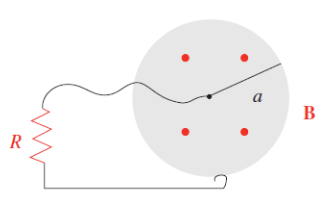
\includegraphics[scale=0.3]{e_10_9_0.png}\\
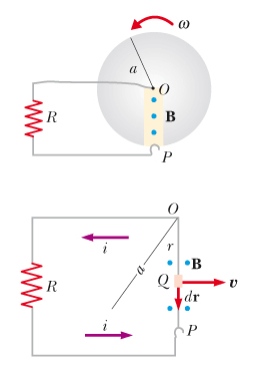
\includegraphics[scale=0.3]{e_10_9_1.png}
\subsubsection*{Formule utilizzate}
\subsubsection*{Soluzione punto a}
$\vec{E_i} = \vec{v}\wedge\vec{B}$\tab\tab$\vec{v} = \omega r\vec{u_\Phi}$\tab\tab$\vec{E_i} = \omega r B \vec{u_r}$\\
$\varepsilon = \oint E_i d\vec{s} = \int \omega rB\vec{u_r}d\vec{r}$\\
$\varepsilon_i = \left[\frac{1}{2}\omega Br^2\right]^a_0 = \frac{1}{2}\omega Ba^2$\\
Alternativamente si può usare il flusso tagliato (l'area spezzata di $d\Theta$ è pari a $\frac{1}{2}d\theta a^2$)\\
$i = \frac{\varepsilon_i}{R} = \frac{\omega Ba^2}{2R} = 0.8 A$\\
Tale corrente circola dal centro verso il bordo come is deduce dalla direzione di $\vec{E_i}$.\\
Vista la presenza di B su un elementino di filo $d\vec{r}$ agisce la forza di Laplace: $d\vec{F} = id\vec{r}\wedge\vec{B}$ \\
Questa forza produce il momento (usando il centro come polo): $d\vec{M_i} = \vec{r}\wedge d\vec{F} = \vec{r} \wedge (id\vec{r}\wedge\vec{B})$\\
Ortogonale al disco e di verso entrante (tende a far ruotare il disco in verso orario).\\
Calcoliamo la forza: $d\vec{F} = id\vec{r}\wedge\vec{B} = \left(\frac{1}{2}\omega Ba^2\right) d\vec{r}\wedge\vec{B} = -\left(\frac{1}{2}\omega Ba^2\right) drB\vec{u_x}$\\
$d\vec{F} = -\frac{1}{2}\omega B^2a^2dr\vec{u_x}$\\
Calcoliamo il momento: $d\vec{M_i} = \vec{r}\wedge d\vec{F} = -\frac{1}{2}\omega B^2a^2rdr \vec{u_z}$\\
$\vec{M} = \int_0^a d\vec{M_i} = -\int_0^a\frac{1}{2}\omega B^2a^2rdr\vec{u_z} = -\left[\frac{1}{2}\omega B^2a^2\frac{r^2}{2}\right]_0^a\vec{u_z} = -\frac{B^2a^4}{4R}\omega\vec{u_z}$
Si tratta di un momento frenante che è proporzionale a $\omega$ quindi di tipo viscoso, detto "momento di attrito elettromagnetico".
\subsubsection*{Soluzione punto b}
Per mantenere in moto di disco bisogna applicare dall'esterno il momento (momento motore) M' = -M e spendere la potenza:\\
$P = \frac{dW}{dt} = \frac{M d\theta}{dt} = M\omega = \frac{B^2a^4}{4R}\omega^2$\\
Che corrisponde alla potenza dissipata per effetto Joule:\\
$P = RI^2 = R\left(\frac{\omega Ba^2}{2R}\right)^2=\frac{\omega^2 B^2a^4}{4R} = 5.06 * 10^{-2}\ W$
\subsubsection*{Soluzione punto c}
Siccome la corrente è costante la carica si trova come:\\
$Q = i \Delta t= 48C$\\
Allo stesso risultato si poteva arrivare con la legge di Felici usando il flusso tagliato:\\
$Q = \frac{Ba^2\theta}{2R} = \frac{Ba^2\omega \Delta t}{2R} = 47.7\ C$
\newpage

\end{document}